\documentclass[aps,prl,twocolumn,showpacs,superscriptaddress,groupedaddress,nofootinbib]{revtex4}  % for review and submission
\usepackage{graphicx}  % needed for figures
\usepackage{dcolumn}   % needed for some tables
\usepackage{bm}        % for math
\usepackage{amsmath,amssymb}   % for math
\usepackage{aas_macros}
\usepackage{multirow}
\usepackage{color}
\usepackage{verbatim}
\usepackage{times}
\newcommand{\mr}{\mathrm}
% avoids incorrect hyphenation, added Nov/08 by SSR
\hyphenation{ALPGEN}
\hyphenation{EVTGEN}
\hyphenation{PYTHIA}
\newcommand{\yr}{\ensuremath{\,{\rm yr}}}
\newcommand{\cm}{\ensuremath{\,{\rm cm}}}
\newcommand{\m}{\ensuremath{\,{\rm m}}}
\newcommand{\km}{\ensuremath{\,{\rm km}}}
\newcommand{\pc}{\ensuremath{\,{\rm pc}}}
\newcommand{\Mpc}{\ensuremath{\,{\rm Mpc}}}
\newcommand{\K}{\ensuremath{\, {\rm K}}}
\newcommand{\mK}{\ensuremath{\, {\rm mK}}}
\newcommand{\psr}{\ensuremath{\,{\rm sr}^{-1}}}
\newcommand{\Hz}{\ensuremath{\, {\rm Hz}}}
\newcommand{\kHz}{\ensuremath{\, {\rm kHz}}}
\newcommand{\MHz}{\ensuremath{\, {\rm MHz}}}
\newcommand{\erg}{\ensuremath{\,{\rm erg}}}
\newcommand{\eV}{\ensuremath{\,{\rm eV}}}
\newcommand{\keV}{\ensuremath{\,{\rm keV}}}
\newcommand{\Jy}{\ensuremath{\,{\rm Jy}}}
\newcommand{\Msun}{\ensuremath{{M_\sun}}}
\newcommand{\Lsun}{\ensuremath{{L_\sun}}}
\newcommand{\Zsun}{\ensuremath{{Z_\sun}}}
\newcommand{\tsec}{\ensuremath{{\rm s}}}
\newcommand{\nur}{\ensuremath{{\nu_R}}}
\newcommand{\nul}{\ensuremath{{\nu_L}}}
\newcommand{\los}{l.o.s.}
\newcommand{\tcb}{\textcolor{blue}}

\begin{document}
% The following information is for internal review, please remove them for submission
\widetext
% the following line is for submission, including submission to the arXiv!!
%\hspace{5.2in} \mbox{Fermilab-Pub-04/xxx-E}

\title{Recovering Lost 21cm Radial Modes via Cosmic Tidal Reconstruction}

\author{Hong-Ming Zhu} 
\affiliation{Key Laboratory for Computational Astrophysics,  National Astronomical Observatories, Chinese Academy of Sciences, 20A Datun Road, Beijing 100012, China}
\affiliation{University of Chinese Academy of Sciences, Beijing 100049, China}

\author{Ue-Li Pen} 
\affiliation{Canadian Institute for Theoretical Astrophysics, 60 St. George Street, Toronto, Ontario M5S 3H8, Canada}
\affiliation{Canadian Institute for Advanced Research, CIFAR Program in Gravitation and Cosmology, Toronto, Ontario M5G 1Z8, Canada}
\affiliation{Perimeter Institute for Theoretical Physics, 31 Caroline St. N., Waterloo, ON, N2L 2Y5, Canada}

\author{Yu Yu}
\affiliation{Key laboratory for research in galaxies and cosmology,
Shanghai Astronomical Observatory, Chinese Academy of Sciences,
80 Nandan Road, Shanghai 200030, China}
\date{\today}

\author{Xuelei Chen}
\affiliation{Key Laboratory for Computational Astrophysics,  National Astronomical Observatories, Chinese Academy of Sciences, 20A Datun Road, Beijing 100012, China}
\affiliation{University of Chinese Academy of Sciences, Beijing 100049, China}
\affiliation{Center of High Energy Physics, Peking University, Beijing 100871, China}

\begin{abstract}
21cm intensity mapping has emerged as a promising technique to map the 
large scale structure of the Universe, at redshifts $z$ from 1 to 10.
Unfortunately, many of the key cross correlations with photo-$z$ galaxies
and the CMB have been thought to be impossible due to foreground
contamination for radial modes with small wavenumbers \tcb{(copied)}. 
These modes are usually subtracted in the foreground subtraction process.
We recover lost 21cm radial modes via cosmic tidal reconstruction and 
find more than 60\% cross correlation signal at $\ell\lesssim100$ and 
even more on larger scales can be recovered from null. 
The tidal reconstruction method opens up a new set of possiblities to 
probe our Universe and is extremely valuable not only for 21cm surveys
but also CMB and photometric redshift observations.
\end{abstract}

\pacs{}
\maketitle

{\it Introduction.}---The current and future cosmological observations aim
to map a large fraction of the Universe with unprecedent precision, varying
from LSST \cite{2009:lsst}, Euclid \cite{2011:euclid}\cite{2012:euclid}, 
Planck mission \tcb{(which paper shall we cite?)}, CMB S4 \tcb{(cite which?)}, 
etc. In addition to these
experiments, 21cm intensity mapping has emerged as a powerful probe of the 
large scale structure of the Universe \cite{2008:21cm}\cite{chang}.
However, the astrophysical foregrounds from galatic and extra-galatic 
synchrotron and free-free emissions are stronger than the cosmological 21cm 
signal by many orders of magnitude. These foregrounds are expected to be 
spectrally smooth, which means they would contaminate small radial
modes, i.e. all modes with low $k_\parallel$.
While there are not many modes with small $k_\parallel$, many other cosmic
observations with broad window functions along the radial direction only 
probe these modes, like weak lensing, photo-$z$ galaxies, 
integrated Sachs-Wolf effect, kinetic Sunyaev-Zel'dovich effect and others.  
Thus this makes it very hard to cross correlate these cosmic probes with 
21cm intensity mapping surveys 
\cite{2007ApJ...660.1030F}\cite{2008MNRAS.384..291A} \tcb{(cite more?)}. 
To study how to solve this problem is of great importance for both 21cm 
intensity mapping surveys and other impartant cosmic surveys.

Recently an new method called {\it cosmic tidal reconstruction} has been 
developed \cite{2012:pen}\cite{2015:zhu}, it can reconstruct the large scale 
tidal field and hence large scale density field from the alignment of small 
scale cosmic structures.
The modes with small $k_\parallel$ and large $k_\perp$ are well 
reconstructed \cite{2015:zhu}, which are exactly those lost in the foreground 
subtraction in 21cm experiments. 
This technique enables the reconstruction of small radial modes, which are 
essential for CMB and other cross correlations.

In this {\emph Letter} we study how to use cosmic tidal reconstruction to 
reconstruct the lost large scale radial modes, and further cross correlate with
CMB lensing, photo-$z$ galaxies and ISW effect. 
We find such reconstruction technique recovers more than 60\% cross correlation 
signal at $\ell\lesssim100$ from nothing and even more at larger scales. 
This opens up a new set of possiblities to understand the origin and evolution
of our Universe.

{\it Cosmic tidal reconstruction.}---Cosmic tides is a new way to view the
tidal effect of gravity on the structure of matter clustering \cite{2012:pen}.
The large scale density field can be reconstructed from the anisotropic tidal 
distortions of the locally measured matter power spectrum with good
accuracy \cite{2012:pen}\cite{2015:zhu}.
The basic idea of purely transverse tidal reconstruction has been studied in
Ref. \cite{2012:pen} and further expanded in Ref. \cite{2015:zhu}.
Here we briefly discuss the physical idea and summarize the process of cosmic
tidal reconstruction. 

The evolution of small scale density perturbations is modulated by long 
wavelength perturbations \cite{2014:tidal}. 
The anisotropic distortions in the local small scale power specturm,
$\propto\hat{k}^i\hat{k}^jt_{ij}^{(0)}$, arise from the coupling of small scale
density fluctuations with the large scale tidal field $t_{ij}$, where 
$t_{ij}=\Phi_{,ij}-\delta_{ij}\nabla^2\Phi/3$, $\hat{\ }$ denotes the 
unit vector and superscript (0) denotes some ``initial'' time. 
While in principle the tidal field $t_{ij}$ has 5 independently observable
components, the two transverse shear terms, 
$(\hat{k}^2_1-\hat{k}^2_2)\gamma_1^{(0)}$ and 
$2\hat{k}_1\hat{k}_2\gamma_2^{(0)}$, 
which describe quadrupolar distortions in the tangential plane perpendicular
to the line of sight, are less affected by peculiar velocities.
Since $\gamma_1=(\Phi_{,11}-\Phi_{,22})/2$ and $\gamma_2=\Phi_{,12}$
only involves derivatives in the tangential plane, the changes in $\gamma_1$
and $\gamma_2$ due to redshift space distortion are expected to be a second
order effect. The two gravitational tidal shear fields $\gamma_1$ and $\gamma_2$
can be converted to the 2D convergence field, 
$\kappa_\mr{2D}=(\Phi_{,11}+\Phi_{,22})$, using
\begin{eqnarray}
\label{eq:kappa2d}
\kappa_{\mr{2D},11}+\kappa_{\mr{2D},22}=
(\gamma_{1,11}-\gamma_{1,22}+2\gamma_{2,12}).
\end{eqnarray}
The 3D convergence $\kappa_\mr{3D}=\nabla^2\Phi/3\propto\delta$ which gives
the large scale density field, can further be obtained from
\begin{eqnarray}
\label{eq:kappa3d}
\kappa_{\mr{3D},11}+\kappa_{\mr{3D},22}=\frac{2}{3}\nabla^2\kappa_\mr{2D}.
\end{eqnarray}
Since only two transverse tidal shear fields $\gamma_1(\bm{x})$ and 
$\gamma_2(\bm{x})$ are used, the change of the large scale density field along
the line of sight is inferred from the variations of $\gamma_1$ and $\gamma_2$
along the $z$ axis. The error of $\kappa_\mr{3D}$ is 
\begin{eqnarray}
\sigma_{\kappa_\mr{3D}}(\bm{k})\propto\big({k^2}/{k_\perp^2}\big)^2,
\end{eqnarray}
which is anisotropic in $k_\perp$ and $k_\parallel$ \cite{2015:zhu}.
The reconstruction works best for modes with low $k_\parallel$ and high 
$k_\perp$, which can not be obtained from 21cm surveys and contribute 
substantially to cosmological observables from other surveys mentioned above.
Thus cosmic tidal reconstruction provides a good opportunity to recover lost 
radial modes and improve the cross correlations.

The tidal reconstrction works as follows. The first step is to convolve
the density field with a Gaussian kernel, $S(\bm{k})=e^{-k^2R^2/2}$, which
filters out the small scale nonlinear structures.
Here we still take $R=1.25\ \mr{Mpc}/h$ \cite{2012:pen}\cite{2015:zhu}.
Next step is to gaussianize the smoothed density field by taking a logarithmic
transform or ranking the density fluctuations into a Gaussian distribution.
In the following reconstruction, we adopt the latter as after the simulated
foreground subtraction, some of the density contrasts becomes smaller than $-1$,
which makes it hard to take the logarithmic transform, $\mathrm{ln}(1+\delta)$.
The gravitational tidal shear fields can be estimated by applying quadratic 
tidal shear estimators $\hat{\gamma}_1$ and $\hat{\gamma}_2$ to the density 
field as in 21cm lensing reconstruction \cite{2008:lu}. 
Then the 3D tidal convergence field $\kappa_\mr{3D}$ is given by the linear 
combination of tidal shear fields using Eq.(\ref{eq:kappa2d}) and 
Eq.(\ref{eq:kappa3d}).
The reconstructed noisy field $\kappa_\mr{3D}$ is related to the original 
density field as 
\begin{eqnarray}
\kappa_\mr{3D}(k_\perp,k_\parallel)=b(k_\perp,k_\parallel)
\delta(k_\perp,k_\parallel)+n(k_\perp,k_\parallel),
\end{eqnarray}
where $b=P_{\kappa_\mr{3D}\delta}/P_{\delta}$ is the bias factor and $n$ is 
the noise of reconstruction \cite{2015:zhu}. 
The reconstructed clean field is given by 
\begin{eqnarray}
\label{eq:kapc}
\hat{\kappa}_c=({\kappa_\mr{3D}}/{b})W,
\end{eqnarray}
where the Wiener filter $W(k_\perp,k_\parallel)=
P_\delta/(P_{\kappa_\mr{3d}}/b^2)$.


{\it Simulation setup.}---We further explore this idea with numerical 
simulations. We employ an ensemble of six $N$-body simulations from the
$\mr{CUBEP}^3\mr{M}$ code \cite{2013:code}. 
Each simulation includes $2048^3$ particles in a $(1.2\mr{Gpc}/h)^3$ box 
with following cosmological parameters: Hubble parameter $h=0.678$, baryon
density $\Omega_{b}=0.049$, dark matter density $\Omega_{c}=0.259$,
amplitude of primordial curvature power spectrum $A_s=2.139\times10^{-9}$ at 
$k_0=0.05\;\mr{Mpc}^{-1}$ and scalar spectral index $n_s=0.968$.
In the following analysis we use outputs at $z=1$.

\begin{figure}[tbp]
\begin{center}
\includegraphics[width=0.48\textwidth]{1.000ratio2d_fswf.eps}
\end{center}
\vspace{-0.7cm}
\caption{The upper panel shows the ratio between the power spectra of the 
foreground subtracted density field and the original density field, i.e. 
$P_{\delta{fs}}/P_\delta$. 
The lower panel shows the ratio between the power spectra of the reconstructed 
field and the original density field, i.e. $P_{\kappa_c}/P_\delta$.
Here we show results for $R_\parallel=60\ \mr{Mpc}/h$.}
\label{fig:ratio}
\end{figure}

We could approximately use dark matter to represent 21cm source distributions.
This is a good approximation since the neutral hydrogen traces the total mass
distribution fairly well at low redshifts. We simply assume the experimental
noise to be zero above a cut off scale and infinity below the cut off scale.
This is a reasonable approximation for a filled aperture experiment, which
has good brightness sensitivity and an exponetially growing noise at small 
scales. \tcb{(above two sentences copied)}
We choose this scale to be $k_c=0.5\ h/\mr{Mpc}$, which corresponds
to $\ell=1150$ at $z=1$. This is realistic for the ongoing 21cm experiments like
CHIME \cite{2014SPIE.9145E..22B}\cite{2014SPIE.9145E..4VN}
and Tianlai \cite{2012IJMPS..12..256C}\cite{2015ApJ...798...40X}.

We are not going to provide a detailed 21cm data reduction process in this 
letter, so we simply  use a high pass filter 
$W_{fs}(k_\parallel)=1-e^{-k_\parallel^2R_\parallel^2/2}$ to simulate the 
foreground subtraction. We show results for the two different scales 
$R_\parallel=60\ \mr{Mpc}/h$ and $R_\parallel=15\ \mr{Mpc}/h$, which gives
$W_{fs}=0.5$ at $k_\parallel=0.02\ \mr{Mpc}/h$ and 
$k_\parallel=0.08\ \mr{Mpc}/h$, respectively. The former is an optimal case, 
i.e. we remove modes for $k_\parallel\lesssim0.02\ \mr{Mpc}/h$ while the latter
is already achieved in the current 21cm observations 
\cite{2013ApJ...763L..20M}\cite{2013MNRAS.434L..46S}.

The observed 21cm field after foreground subtraction is given by 
\begin{eqnarray}
\delta_{fs}(\bm{k})=\delta(\bm{k})W_{fs}(k_\parallel)\Theta(k_c-k),
\end{eqnarray}
where $\delta(\bm{k})$ is the density field from simulations, $W_{fs}$ accounts
the effect from foreground subtraction and $\Theta(x)$ is the step function 
which equals $1$ for $x\ge0$ and otherwise $0$.
Then we get the reconstructed clean field $\kappa_c$ from $\delta_{fs}$ via
cosmic tidal reconstruction. In Fig.\ref{fig:ratio}, the upper panel shows the 
ratio between $P_{\delta_{fs}}$ and $P_{\delta}$ and the lower panel shows the
ratio between $P_{\kappa_c}$ and $P_\delta$ for $R_\parallel=60\ \mr{Mpc}/h$. 
We find the lost radial modes appears again in the reconstructed field.

{\it Cross correlation signal.}---To show how much the cross correlations is 
improved by cosmic tidal reconstruction and study the dectability of the
cross correlations, we need to generate the lensing convergence field,
the angular distribution of photo$-z$ galaxies and the temperature fluctuation
due to the ISW effect from $N$-body simulations.

\begin{figure}[tbp]
\begin{center}
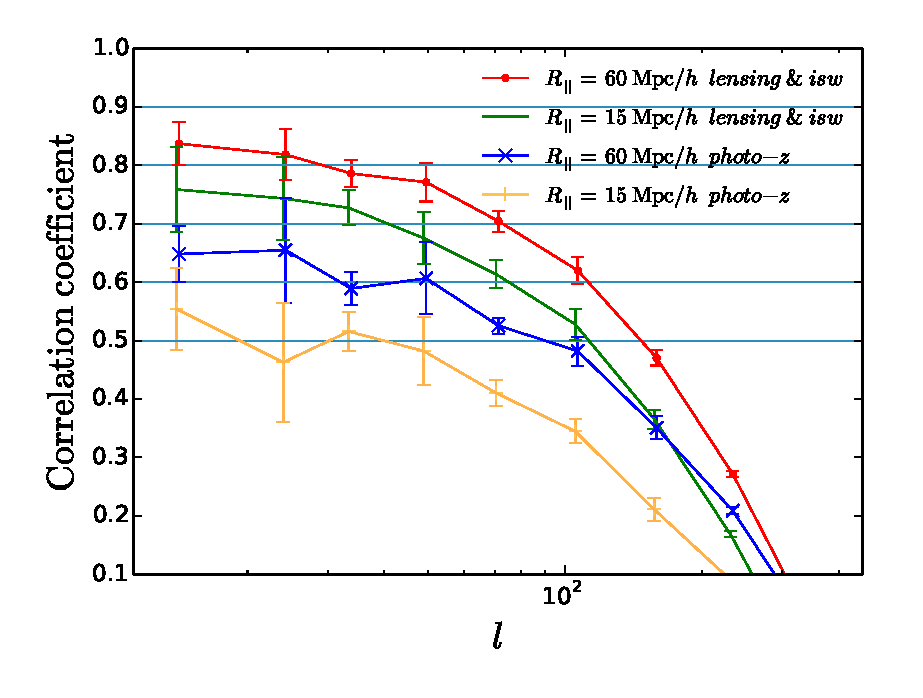
\includegraphics[width=0.48\textwidth]{fig1b.eps}
\end{center}
\vspace{-0.7cm}
\caption{Cross correlation coefficients.}
\label{fig:cc}
\end{figure}

%\begin{figure}[tbp]
%\begin{center}
%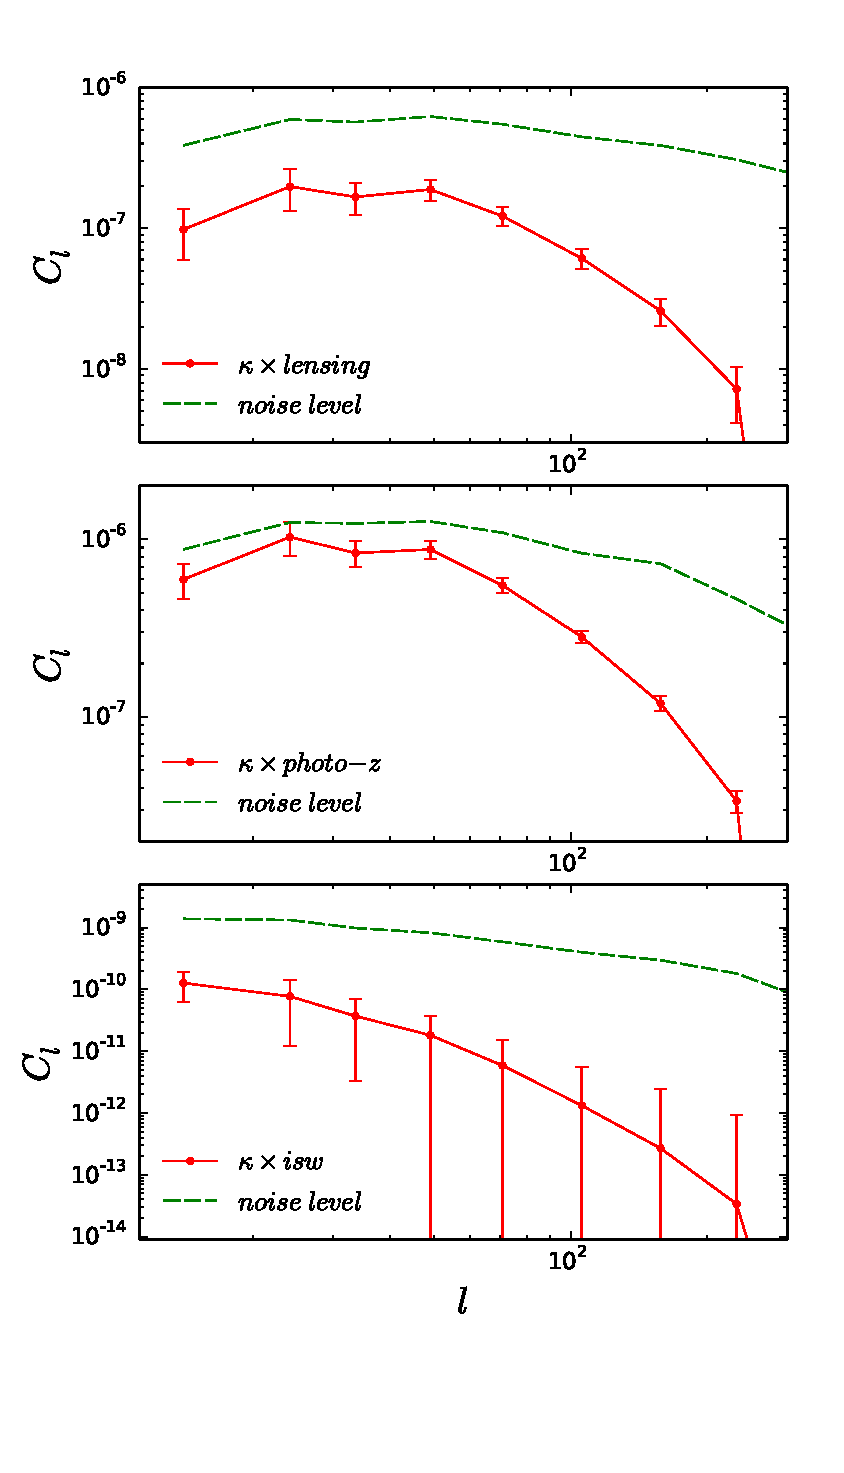
\includegraphics[width=0.48\textwidth]{f8.eps}
%\end{center}
%\vspace{-0.7cm}
%\caption{The cross correlation signals between 21cm and other cosmic probes.}
%\end{figure}

(1) CMB lensing.---The weak lensing convergence is a weighted projection
of the dark matter fluctuation along line-of-sight to the last scatter surface,
\begin{eqnarray}
\kappa(\bm{\theta})=\int_0^{\chi_s}d\chi 
W(\chi)\delta(\chi\bm{\theta},\chi)\ ,
\end{eqnarray}
where the lensing kernel
\begin{eqnarray}
W(\chi)=\frac{3}{2}\Omega_{m0}H_0^2a^{-1}\chi\frac{\chi_s-\chi}{\chi_s}\ ,
\end{eqnarray}
with $\chi_s=\chi(z_s=1090)$.
To generate the convergence field from simulation data, we first squeeze the 
simulation box to a 2D plane, then multiply the $W(\chi)$, as the lensing
weight is a slow varying function for the case of CMB lensing.
Then we obtain the 2D convergence field contributed by the simulated density.

(2) Photometry survey.---We calculate the projected galaxy density field 
at $z\sim 1$ with usual photo-$z$ bin width of $0.2$, i.e. $z^P\in(0.9,1.1)$. 
We adopt the galaxy distribution characterized by 
$n^P(z^P)dz^P\propto z^{P,\alpha}\mr{exp}[-(z^P/z^{*})^\beta]$
with $\alpha=2$, $z^*=0.5$, $\beta=1$
and assume the photo-$z$ scatter $P(z^P|z)$ is perfectly known to be in a Gaussian form with photo-$z$ error $\sigma_P=0.05(1+z)$.
The 2D angular galaxy distribution is given by
\begin{eqnarray}
\delta_\mr{2D}(\bm{\theta})=\int_0^\infty dzW(z)
\delta(\chi\bm{\theta},\chi(z))\ ,
\end{eqnarray}
where the window function 
\begin{eqnarray}
W(z)=\int_{0.9}^{1.1}P(z^P|z) n^P(z^P) dz^P\ . 
\end{eqnarray}

(3) ISW effect.---ISW is the observed CMB temperature fluctuations induced by the integral of the late-time potential variation
\begin{eqnarray}
\frac{\Delta T}{T}(\bm\theta)=2\int \dot\Phi(\bm{\theta},t)dt\ .
\end{eqnarray}
In Fourier space, approximating that the evolution of the overdensity field with time is given by linear theory
$\dot\delta(\bm{k},t)=\dot D(t)\delta(\bm{k},t=0)$, we have
\begin{eqnarray}
\dot\Phi(\bm{k},t)=\frac{3}{2}\Omega_{m0}\frac{H_0^2}{k^2}\frac{\delta(\bm{k},t)}{a(t)}H(t)(1-\beta(t))\ ,
\end{eqnarray}
where $\beta(t)=d\ln D(t)/d\ln a(t)$ and $D(t)$ is the growth factor.
In our implementation, we also approximate the $\beta(t)$ as a constant across the simulation box.


\begin{figure}[tbp]
\begin{center}
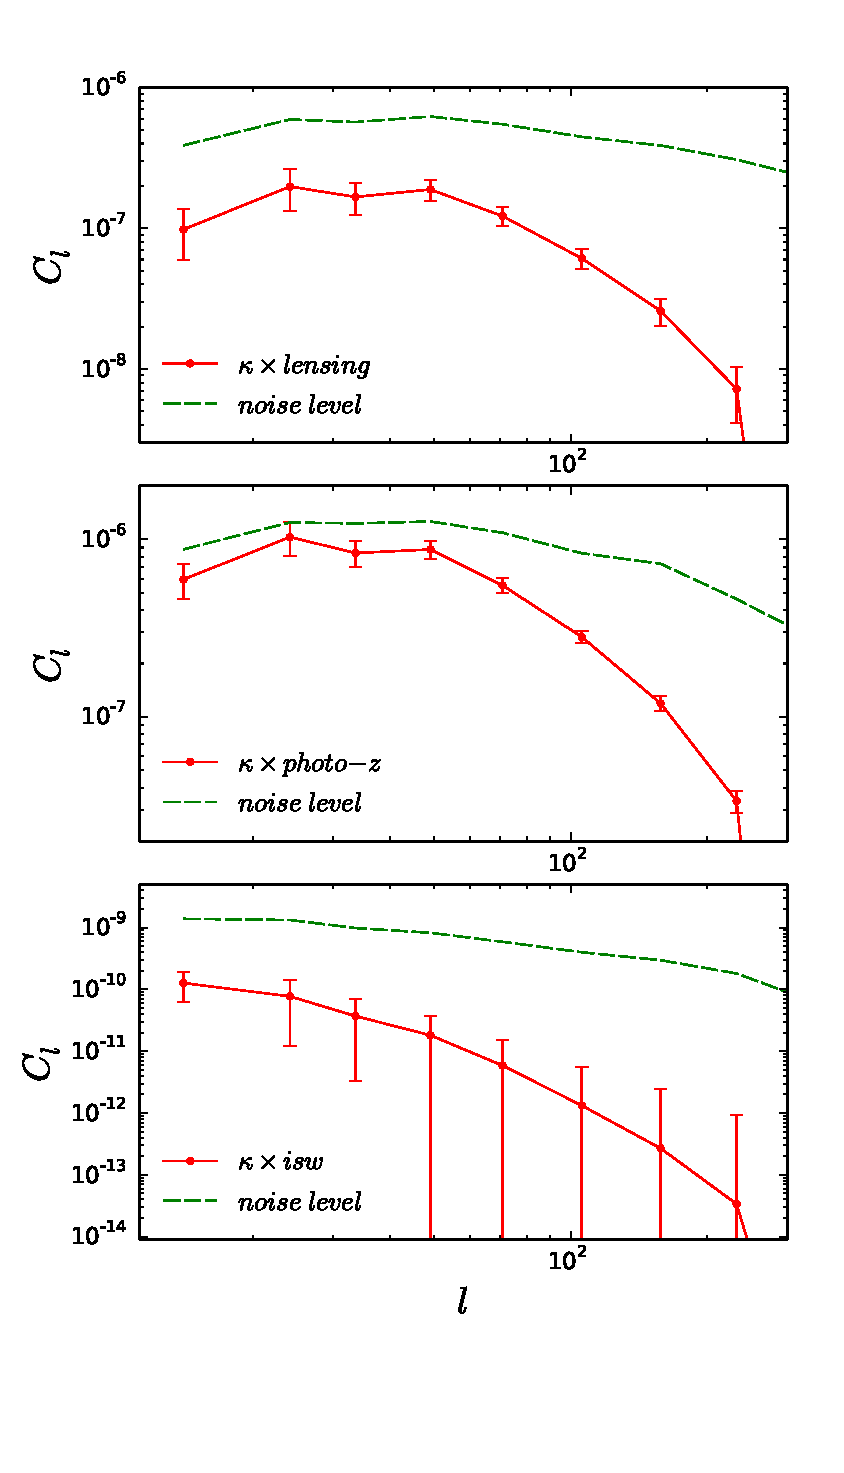
\includegraphics[width=0.48\textwidth]{f8.eps}
\end{center}
\vspace{-1.9cm}
\caption{The cross correlation signal between 21cm and other cosmic probes for
$R_\parallel=60\ \mr{Mpc}/h$.}
\label{fig:cs}
\end{figure}

In Fig. \ref{fig:cc}, we show the cross correlation coefficients for 21cm with 
different observations for both $R_\parallel=60\ \mr{Mpc}/h$ and 
$R_\parallel=15\ \mr{Mpc}/h$. Due to the similar treatment of CMB lensing field
and the ISW field, we get the same correlation coefficient for them. 
The correlation coefficient for photo-$z$ galaxies is smaller than the other
two since we use a narrow bin which locates at $z=1$ with bins width $0.2$.

In Fig. \ref{fig:cs}, we show the three cross correlation signals and the noise
levels for the signal \tcb{(is the green curve called noise level?)}. The error
on the signal is given by
\begin{eqnarray}
\sigma_{C_\ell}=\frac{1}{(2\ell+1)\Delta_\ell f_\mr{sky}}
{(C_\ell^{\alpha\beta})^2+(C_\ell^{\alpha}+n_\ell^{\alpha})
(C_\ell^{\beta}+n_\ell^{\beta})}.
\end{eqnarray}
For the 21cm field, $n_\ell^\mr{21cm}$ is given through Eq.(\ref{eq:kapc}). 
The noise for CMB lensing is assumed to be the same as $Planck\ 2015$ results 
\cite{2015:plancklensing}. For ISW effect, $n_\ell^\mr{ISW}$ is the large scale
CMB power spectrum $C_\ell^{TT}$. We choose $f_\mr{sky}$ to be $0.25$ for 
CMB lensing and photo-$z$ galaxies, and $1$ for the ISW effect. We find by
using cosmic tidal reconsruction, we are able to detect the cross correlation
signals with ongoing 21cm experiments \cite{2014SPIE.9145E..22B,2014SPIE.9145E..4VN,2012IJMPS..12..256C,2015ApJ...798...40X}. 
The redshift information contained in 21cm observations allows us to constrain
the expansion history of the Universe by cross correlating with the ISW effect.
The detectability for ISW effect can be further improved by including CMB 
polarization data \cite{2011PhRvD..83f3001L}.

{\it Discussion.}---It may seem to be odd that the modes lost appear again
after reconstruction. This can be undertanded intuitively.
The reconstructed field $\kappa_c$ is given by the linear combination of 
quadratic estimators, in the form of 
$\kappa_c(\bm{x})\sim\delta_{fs}(\bm{x})\delta_{fs}(\bm{x})$. In Fourier 
space this can be written as $\kappa_c(\bm{k})\sim\int d^3k'
\delta_{fs}(\bm{k}')\delta_{fs}(\bm{k}-\bm{k}')$, i.e. the reconstructed 
field is given by the convolution of $\delta_{fs}(\bm{k}')$ and 
$\delta_{fs}(\bm{k}-\bm{k}')$. Although $\delta_{fs}$ has no small radial
nodes, i.e. $k_{\parallel}'$ and $k_\parallel-k_{\parallel}'$ can not be small,
$k_\parallel$ can reach the low $k_\parallel$ regime.
Here we extract the information about matter distribution on large scales 
contained in the small scale matter distributions. The power spectrum of 
$\kappa_c$ is give by the connected four point function of $\delta_{fs}$,
which means we are using the information that comes from higher order statistics
and is not included in the two point statistics of $\delta_{fs}$, i.e. 
power spectrum.

The tidal shear estimators used is optimal for Gaussian sources and in the 
long wavelength limit \cite{2015:zhu}.
The results can still be improved by constructing optimal tidal shear 
estimators for non-Gaussian sources as in 21cm lensing \cite{2010:lu} and 
considering the general case. This means here we present the ``least optimal''
case of recovering the cross correlation signals and even better results can be
achieved in future.

The BAO reconstruction technique \cite{2007:bao} has been shown to be still
useful in 21cm surveys \cite{2015:bao1}\cite{2015:bao2}. While there are not 
many modes with small $k_\parallel$ lost in the foreground subtraction, the 
differential motions which smear the BAO peaks are substantially contributed
by large scale modes with $k\lesssim0.1\ h/\mr{Mpc}$ \cite{2007:bao}.
The tidal reconstruction compensates the foreground wedge at low $k_\parallel$
and high $k_\perp$ and hence can further improve the BAO reconstruction in 
21cm surveys. Since all cosmological 21cm experiments share the same foreground
problem, no matter low redshift surveys for BAO or high redshift observations
for the EOR signal, the tidal reconstruction can also help high redshift cross 
correlations like the 21cm-kSZ signal from EOR \cite{2015:marcelo}. Based
on above discussions, we conclude that cosmic tidal reconstruction is extremely
valuable for all cosmological 21cm surveys as well as CMB and photometric
redshift observations.

We acknowledge helpful discussions with Marcelo Alvarez, Alex van Engelen,
Philippe Berger, Yi-Chao Li and Shifan Zuo.
Our simulation computations were performed on the BlueGene/Q supercomputer 
located at the University of Toronto’s SciNet HPC facility.
SciNet is funded by the CFI under the auspices of Compute Canada, 
the Government of Ontario, the Ontario Research Fund – Research Excellence;
and the University of Toronto.
We acknowledge the support of the Chinese MoST 863 program under Grant 
No. 2012AA121701, the CAS Science Strategic Priority Research Program 
XDB09000000, the NSFC under Grant No. 11373030 and 11403071, IAS at 
Tsinghua University, CHEP at Peking University, and NSERC.

\bibliographystyle{apsrev}
\bibliography{cro}

\end{document}
